Long short-term memory networks are very similar to recurrent neural networks, but they address the issue of gradient approximation by introducing memory cells and a cell state \citep{hochreiter1997long}. A visualization of these networks is shown in Figure \ref{fig:LSTM}. The cell state acts as the `long term' memory, making use of all previous information. The only increase that can occur within the cell state is additive, which limits the impact of long-term dependencies that caused issues within RNNs. The memory cells act as the `short term' memory, making use of mostly the current input and previous output.

\begin{figure}[ht]
    \centering
    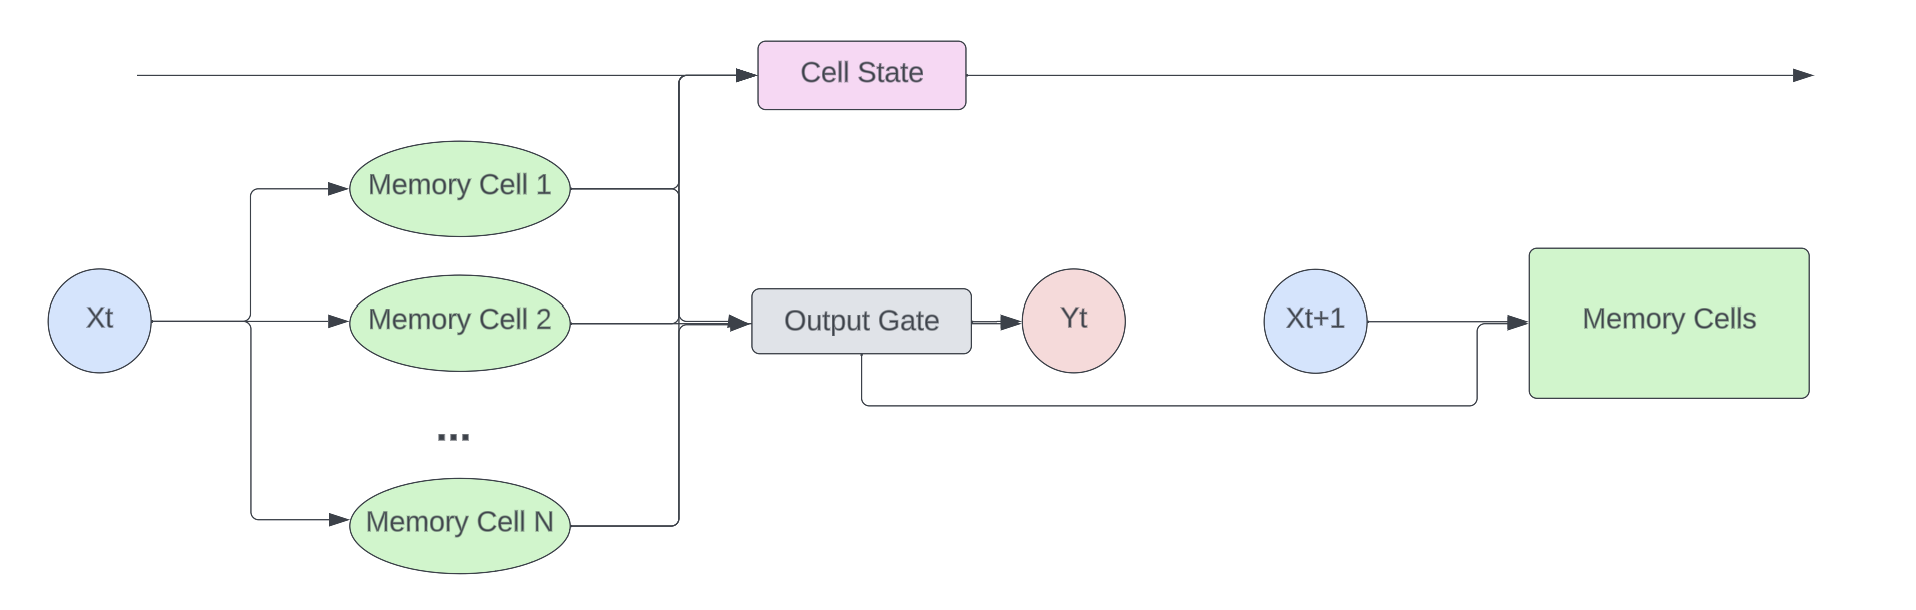
\includegraphics[width=0.9\linewidth]{"Figures/LSTM_Architecture.png"}
    \caption{A visualization of long short-term memory networks.}
    \label{fig:LSTM}
\end{figure}

\begin{figure}[ht]
    \centering
    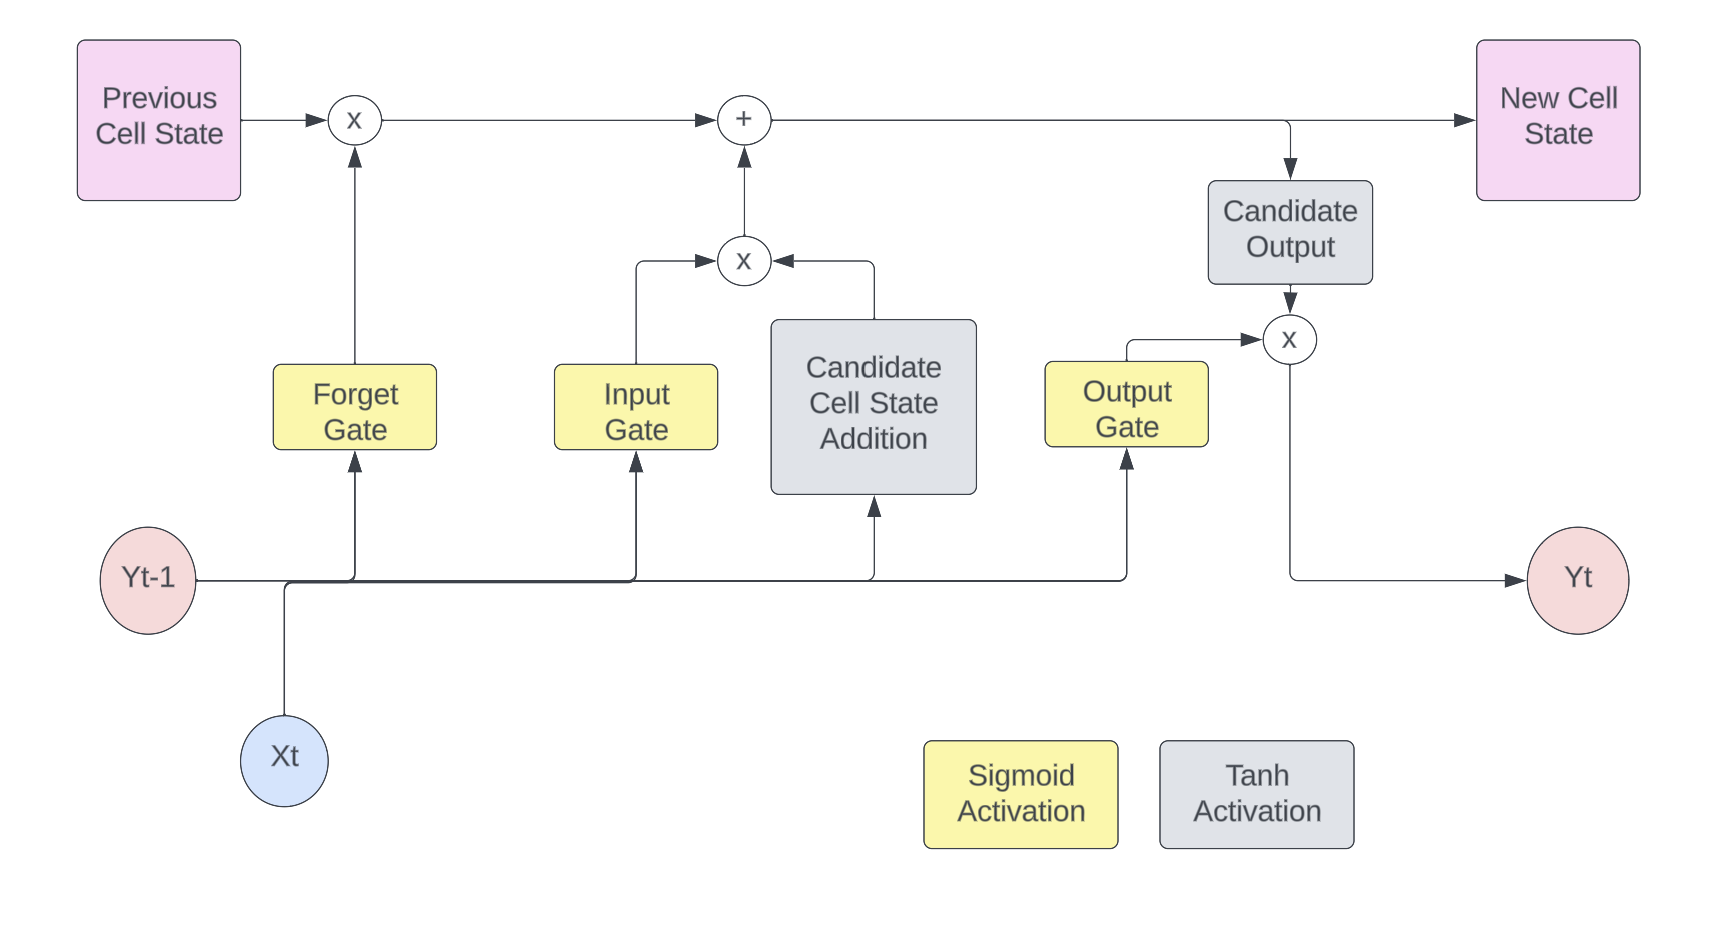
\includegraphics[width=0.9\linewidth]{"Figures/LSTM_Memory_Cell.png"}
    \caption{A visualization of the memory cells in LSTMs.}
    \label{fig:MemoryCells}
\end{figure}

The memory cells are more involved than the typical hidden states of RNNs (see Figure \ref{fig:MemoryCells}). This is because of the way each prediction is used for both the long-term and short-term memory. The current input $x_t$ and previous output $y_{t-1}$ are used in more ways than simply getting the next prediction. The forget gate determines what percentage of the previous cell state is remembered. By using a sigmoid activation function, the forget gate value will be between 0 and 1. Gates function as filters, determining what percentage of the input should actually be kept in the output. Sigmoid activations work well here as they map any values on the real number line to a value between 0 and 1. The cell state is then modified based on the candidate cell state addition, which is then multiplied by the input gate value. This gate acts similarly to the forget gate in the sense that it determines what percentage of the candidate cell state addition is actually added to the cell state. Finally, the cell state is fed into a hyperbolic tangent activation and multiplied by the output gate to determine that final output value $y_t$. The purpose of using the hyperbolic tangent activation is that it allows the output to be positive or negative based on if it is an increase or a decrease, respectively.

Mathematically, the memory cell can be written in notation used previously (adapted from \cite{understandinglstm}). See Table \ref{tab:MemoryCellEquations} for the full equations. The forget gate $f_t$ makes use of a sigmoid activation and has its own corresponding weights and bias, denoted $W_f$ and $b_f$, respectively. The input gate $i_t$ functions similarly, with the notation of a subscript $i$. The new candidate values $\tilde{C_t}$ to be added to the cell state use a hyperbolic tangent activation with the subscript $c$ on the weights and bias. The updated cell state $C_t$ is the product of the forget gate $f_t$ and the previous cell state $C_{t-1}$ plus the new candidate cell state values $C_{t}$ multiplied by the input gate $i_t$. Similar to previously mentioned gates, the output gate $o_t$ uses a sigmoid activation with the subscript $o$ on the weights and bias. The output value $y_t$ is calculated as a proportion (determined by the output gate) of the new cell state.

\begin{table}[hbt!]
\centering
\begin{tabular}{|c|c|p{0.35\linewidth}|}
    \hline 
    Name & Equation  & Purpose\\
    \hline
    Forget Gate & $f_t = \sigma[W_f(y_{t-1}, x_t) + b_f]$ & Determines what proportion of past information can be `forgotten' within the Cell State.\\
    \hline
    Input Gate & $i_t = \sigma[W_i(y_{t-1}, x_t) + b_i]$ & Determines what proportion of current information should be added to the Cell State.\\
    \hline
    New Candidate Value & $\tilde{C_t} = \tanh[W_c(y_{t-1}, x_t) + b_c]$ & Determines what value should be added to the Cell State.\\
    \hline 
    Updated Cell State & $C_t = f_t\cdot C_{t-1} + i_t\cdot \tilde{C_t}$ & Combination of Previous Cell State and Current Cell State to get the New Cell State.\\
    \hline
    Output Gate & $o_t = \sigma[W_o(y_{t-1}, x_t) + b_o]$ & Determines what proportion of the New Cell State should be used as the current prediction.\\
    \hline
    Output Value & $y_t = o_t\cdot \tanh[C_t]$ & A proportion of the New Cell State to be used as a current prediction.\\
    \hline
\end{tabular}
\caption{A table of equations corresponding to each gate and node within Figure \ref{fig:MemoryCells}.}
\label{tab:MemoryCellEquations}
\end{table}
